\documentclass[aspectratio=169]{beamer}
\beamertemplatenavigationsymbolsempty
\usepackage{tcolorbox}
\usepackage{t1enc}
\usepackage[magyar]{babel}
\usepackage[utf8]{inputenc}

%\setbeamertemplate{navigation symbols}{}%remove navigation symbols

\usepackage{fontspec}
%\setmainfont[Mapping=tex-text]{Bebas Neue}
\setmainfont[Mapping=tex-text]{Asap}
\let\sfdefault\rmdefault

\AtBeginSection[]

%\usetheme{Warsaw}
\usecolortheme{frigatebird}
%\usetheme{Szeged}

\tcbset{%
    noparskip,
    colback=noir!90, %background color of the box
    colframe=gray!40, %color of frame and title background
    coltext=blanc, %color of body text
    coltitle=black, %color of title text 
    fonttitle=\bfseries,
    alerted/.style={coltitle=red, 
                     colframe=gray!40},
    example/.style={coltitle=black, 
					 colframe=myOrange!100,},
%                     colback=green!5},
    }

\newfontfamily\bebasfont{Bebas Neue}

%Information to be included in the title page:
%\title{\bebasfont 3 hónap:\ 3 use-case WireGuard-dal}
\title{EMUSEREMA Multiprotocol Session and Redirect Manager}
\author{Szabó Endre}
\institute[HSBP Meetup]{Hackerspace Budapest Online Meetup}
\date[\today]{2020. július 11.}

\begin{document}

{
%\setbeamercolor{background canvas}{bg=violet}
\frame{\titlepage}
}

\section{Áttekintés}
\subsection{terjedelem}

\begin{frame}{A projektről}

	Mi ez?
		\pause
		\begin{itemize}
			\item Egy Python program.
				\pause
			\item Mindenféle remote access protocol sessionjeinek managelésére.
		\end{itemize}
	Miért ez a név?
			\pause
		\begin{itemize}
			\item Rekurzív rövidítés:
				\pause
			\only<1-5>{\item \textcolor{orange}{[A-Z]}MUSEREMA Multiprotocol Session and Redirect Manager}
				\pause
			\only<6>{\item \textcolor{orange}{[A-Z]MU}SEREMA \textcolor{orange}{Mu}ltiprotocol Session and Redirect Manager}
				\pause
			\only<7>{\item \textcolor{orange}{[A-Z]MUSE}REMA \textcolor{orange}{Mu}ltiprotocol \textcolor{orange}{Se}ssion and Redirect Manager}
				\pause
			\only<8>{\item \textcolor{orange}{[A-Z]MUSERE}MA \textcolor{orange}{Mu}ltiprotocol \textcolor{orange}{Se}ssion and \textcolor{orange}{Re}direct Manager}
				\pause
			\only<9->{\item \textcolor{orange}{[A-Z]MUSEREMA} \textcolor{orange}{Mu}ltiprotocol \textcolor{orange}{Se}ssion and \textcolor{orange}{Re}direct \textcolor{orange}{Ma}nager}
				\pause
			\only<1->{\item Kiválóan kereshető:}
				\pause
		\end{itemize}
			\begin{center}
			\only<1->{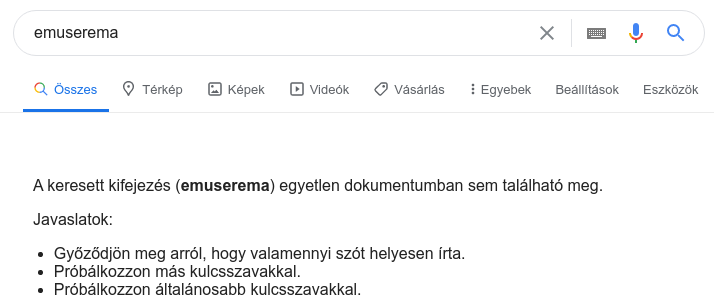
\includegraphics[scale=0.3]{google-0hit.png}}
			\end{center}


\end{frame}

\begin{frame}{Multiprotocol?}
	Többféle protokoll és kliens támogatása:
	\pause
		\begin{itemize}
			\only<1-2>{\item SSH}
	\pause
			\only<3->{\item SSH, kliensek: OpenSSH, PuTTY}
	\pause
\only<1-4>{\item RDP}
	\pause
\only<5->{\item RDP, kliensek: xfreerdp, \texttt{mstsc.exe}}
	\pause
\only<1-6>{\item VNC}
	\pause
\only<7->{\item VNC, kliens: RealVNC\texttrademark}
	\pause
\only<1-8>{\item Weboldal URL-ek}
	\pause
\only<9->{\item Weboldal URL-ek: statikus ``bookmark'' weboldalt generál}
	\pause
			\item (SSH over SCB, nagyon specifikus konstellációban)
		\end{itemize}
\end{frame}

\begin{frame}{Session?}
		\begin{center}
		Mi a session?
		 \end{center}
\end{frame}

\begin{frame}{Session?}
			\begin{center}

				 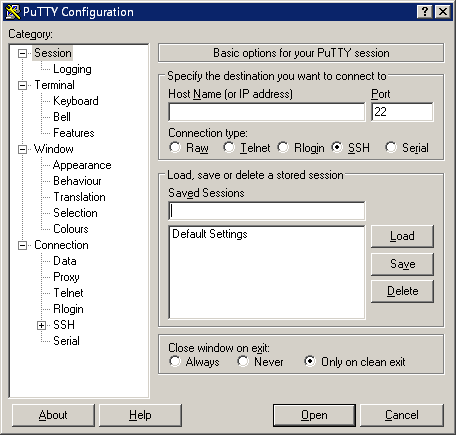
\includegraphics[scale=0.4]{putty.png}
		\pause

		Yay, PuTTY :/

			 \end{center}
\end{frame}

\begin{frame}{Session?}
			\begin{center}

				 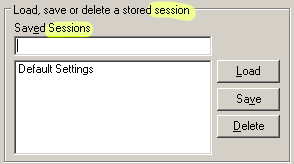
\includegraphics[scale=0.4]{putty-zoom.png}

		\pause

		Na, ez a ``session''.

			 \end{center}
\end{frame}

\begin{frame}[fragile]{Redirect?}


	Redirect: Protokollok automatikus ``egymásba fűzése''.

	\pause

	Példa: SSH-n át elért weboldalak és VNC szerver konfigurációja:

	\pause

	\begin{verbatim}
    Host hubud0xivsh01.y7.hu
        [...]
        # EMUSEREMA added implicit redirection for service \
        # huszb1xirtr01.y7.hu" at URL: http://62.165.209.130
        LocalForward = 44.128.195.255:38023 62.165.209.130:80
        # EMUSEREMA added implicit redirection for service \
        # "hubud0xanrd01.y7.hu web mgmt" at URL: http://44.128.131.98:1880
        LocalForward = 44.128.195.255:38020 44.128.131.98:1880
        # EMUSEREMA added implicit redirection for service \
        # "x VNC" at 44.128.128.3:0
        LocalForward = 44.128.195.255:38019 44.128.128.3:5900

\end{verbatim}
\end{frame}

\begin{frame}{``One more thing\ldots''}

	Bónusz killer feature:

	\pause

	EMUSEREMA mint Ansible inventory plugin:
	\pause
		\begin{itemize}
			\item Minden Ansible futtatáskor kiértékelődik
			\pause
			\item Beépített \texttt{group\_vars} és \texttt{host\_vars} támogatás
		\end{itemize}
\end{frame}

\begin{frame}{Tervezési célok}
	Tervezési célok:
		\pause
	\begin{itemize}
		\item YAML include: \texttt{git submodule} támogatás
		\pause
		\item Moduláris felépítés, dinamikus függőségek
		\pause
		\item Rugalmas attribútum öröklődés
	\end{itemize}
\end{frame}

\begin{frame}{Működése nagyvonalakban}
	Standalone futtatás során
	\pause
	\begin{itemize}
		\item YAML bemeneti file(oka)t dolgoz fel
		\pause
		\item Ezeken feldolgozás előtt rekurzív Jinja2 templating lehet
		\pause
		\item (Feldolgozás)
		\pause
		\item Kimeneti render pluginek elkészítik a kimeneteket
	\end{itemize}
\end{frame}

\begin{frame}[plain]
    \fontsize{50}{60} \bebasfont{Demo}
\end{frame}


\end{document}

